\documentclass[conference]{IEEEtran}
\IEEEoverridecommandlockouts
% The preceding line is only needed to identify funding in the first footnote.

\usepackage{cite}
\usepackage{amsmath,amssymb,amsfonts}
\usepackage{booktabs}
\usepackage{array}
\usepackage{graphicx}
\usepackage{listings}
\usepackage{textcomp}
\usepackage{xcolor}
\usepackage{placeins}
\usepackage{hyperref}
\usepackage{tikz}
\usetikzlibrary{shapes,arrows,positioning,calc}

\def\BibTeX{{\rm B\kern-.05em{\sc i\kern-.025em b}\kern-.08em
    T\kern-.1667em\lower.7ex\hbox{E}\kern-.125emX}}

\lstset{
  basicstyle=\ttfamily\scriptsize,
  breaklines=true,
  breakatwhitespace=true,
  breakautoindent=false,
  breakindent=0pt,
  columns=fullflexible,
  frame=single,
  framerule=0.4pt,
  framesep=2pt,
  linewidth=\linewidth,
  xleftmargin=0pt,
  xrightmargin=0pt,
  aboveskip=0.35\baselineskip,
  belowskip=0.35\baselineskip,
  showstringspaces=false
}

% Table helpers for IEEE two-column layouts (wrap long text instead of cutting it off)
\newcolumntype{L}[1]{>{\raggedright\arraybackslash}p{#1}}
\newcolumntype{C}[1]{>{\centering\arraybackslash}p{#1}}

\begin{document}

\title{Data Disclosure in Artificial Intelligence and Machine Learning Systems: A Systematic Review}

\author{\IEEEauthorblockN{Miguel Rodrigues}
\IEEEauthorblockA{\textit{Department of Computer Science} \\
\textit{ISEP} \\
Porto, Portugal \\
1181734@isep.ipp.pt}}

\maketitle

\begin{abstract}
Data disclosure in machine learning systems poses substantial privacy risk for both organizations and individuals. This systematic review synthesizes empirical evidence on disclosure attacks and mitigation techniques in AI/ML systems across domains, with particular attention to educational applications. Following PRISMA 2020 guidelines~\cite{prisma2020}, we searched IEEE Xplore, ACM Digital Library, Scopus, and Google Scholar for peer-reviewed studies published between January 2018 and January 2026. We identify and characterize three major categories of disclosure threats: membership inference~\cite{shokri2017membership}, model inversion~\cite{fredrikson2015model}, and training data extraction in large language models~\cite{carlini2021extracting}. Corresponding defenses include differential privacy~\cite{abadi2016deep}, federated learning, secure aggregation, and secure multi-party computation. Across the 29 included empirical studies, the evidence suggests that combining statistical and cryptographic controls can provide complementary protection, although privacy--utility trade-offs remain pervasive. Key gaps include limited public benchmarks, heterogeneous privacy metrics, and comparatively sparse research in educational and other specialized domains.
\end{abstract}

\begin{IEEEkeywords}
Privacy leakage, data disclosure, membership inference, model inversion, training data extraction, differential privacy, federated learning, systematic review
\end{IEEEkeywords}

\section{Introduction}

\subsection{Rationale}
Machine learning systems are increasingly trained and deployed on sensitive data---from healthcare records to student academic performance---creating an inherent tension between model utility and individual privacy. Training and serving such models can expose private information through model outputs, intermediate representations, or distributed updates.

Disclosure risks arise through multiple attack vectors. Membership inference determines whether a specific record was included in a model's training set~\cite{shokri2017membership}. Model inversion reconstructs sensitive attributes or training examples from model behavior~\cite{fredrikson2015model}. Training data extraction, particularly acute in large language models (LLMs), can recover verbatim sequences via carefully crafted prompts~\cite{carlini2021extracting}. In practice, these risks are amplified when sensitive content is processed by third-party ML services with unclear retention or training policies.

In parallel, privacy-preserving machine learning (PPML) has matured considerably. Differential privacy (DP) introduces calibrated randomness to limit the influence of any single record while preserving aggregate utility~\cite{abadi2016deep}. Federated learning (FL) supports collaborative training without centralizing raw data, while secure aggregation and secure multi-party computation can reduce server-side visibility of client updates.

\subsection{Scope Definition}
This review focuses specifically on \textbf{training data leakage} through machine learning models and their outputs. We include:
\begin{itemize}
  \item Membership inference (inferring whether a record was used in training)
  \item Model inversion (reconstructing training examples or sensitive attributes)
  \item Training data extraction (recovering verbatim or near-verbatim sequences)
  \item Gradient inversion and related inference attacks in distributed learning
\end{itemize}

We explicitly exclude:
\begin{itemize}
  \item Data breaches or access-control failures outside the model scope
  \item Governance- or anonymization-only work without empirical ML evaluation
  \item Model intellectual property protection (model stealing) when not tied to training-data disclosure
  \item Static data storage security mechanisms unrelated to model leakage
\end{itemize}

\subsection{Objectives and PICOS Framework}
This review follows PRISMA 2020 guidelines and adopts the \textbf{PICOS} framework to ensure transparency and reproducibility.

\noindent\textbf{Population / Problem (P).} AI/ML systems trained or deployed on personal, sensitive, or confidential data, including (but not limited to) healthcare, finance, and education.

\noindent\textbf{Intervention (I).} Methods aimed at (a) assessing disclosure risk through empirical attacks (e.g., membership inference, model inversion, training-data extraction), or (b) mitigating disclosure through technical controls (e.g., DP, FL, secure aggregation, SMPC, HE, private knowledge distillation).

\noindent\textbf{Comparator (C).} Baseline models without privacy protection, alternative privacy mechanisms, or different privacy parameter configurations.

\noindent\textbf{Outcomes (O).} Primary: quantitative privacy metrics (e.g., attack success rates, privacy budgets $\varepsilon/\delta$). Secondary: model utility metrics (accuracy, F1-score, AUC-ROC), computational overhead, and deployment feasibility.

\noindent\textbf{Study Design (S).} Peer-reviewed empirical studies (journal or conference papers) published between 2018 and 2026 reporting experimental evaluation of disclosure risk and/or privacy-preserving techniques using real or synthetic datasets.

\noindent\textbf{Research questions.}
\textit{RQ1 (Typology of risks): What types of data disclosure risks have been identified in AI/ML systems (including educational applications) between 2018 and 2026?}
\textit{RQ2 (Mitigation and trade-offs): Which approaches have been proposed to measure and mitigate disclosure in AI/ML models, and what are their reported impacts on utility and deployment?}

\subsection{Overview of the Existing Literature}
Across the reviewed literature, three attack categories dominate: membership inference, model inversion, and training data extraction. Defenses cluster around statistical mechanisms (notably differential privacy), distributed learning paradigms (federated learning), and cryptographic protections (secure aggregation, SMPC, and variants of homomorphic encryption). Despite rapid progress, results are often difficult to compare due to heterogeneous threat models, datasets, and privacy metrics.

\subsection{Ethical and Sector-Specific Considerations}
The educational sector is a particularly salient application domain. Student data may include academic performance, behavioral traces, learning diagnostics, and, in some systems, biometric identifiers. Educational institutions increasingly deploy AI-driven personalization, automated assessment, and predictive analytics. These uses heighten privacy concerns due to students' vulnerability, the sensitivity of educational records, and regulatory requirements under FERPA (U.S.), GDPR (EU), and related national data-protection frameworks.

\subsection{Structure of the Article}
The remainder of this paper is organized as follows. Section~\nameref{sec:Methods} describes the review methodology. Section~\nameref{sec:Results} presents the selected studies and synthesizes findings by threat and defense categories. Section~\nameref{sec:Conclusion} summarizes key insights and outlines directions for future work.

\section{Methods}
\label{sec:Methods}

\subsection{Protocol and Registration}
This systematic review was conducted following the PRISMA 2020 guidelines and checklist~\cite{prisma2020}. Although the protocol was not pre-registered, it was defined \textit{a priori} before searching, screening, and synthesis.

\subsection{Eligibility Criteria}
We included peer-reviewed empirical studies published between 2018 and 2026 that explicitly evaluate disclosure risk (attacks) and/or mitigation (defenses) in AI/ML systems. We excluded theses, technical reports, and purely theoretical proposals without empirical evaluation.

\subsection{Information Sources}
We searched three academic databases and sources: IEEE Xplore, ACM Digital Library, and Google Scholar.

\subsection{Search Strategy}
We conducted searches in January 2026. Due to the high volume of initial results, we refined the search strategy to focus on document titles for IEEE and ACM to ensure relevance.

\textbf{IEEE Xplore (22 records):} Query applied to 'Document Title': \texttt{("membership inference" OR "model inversion" OR "training data extraction" OR "data disclosure") AND ("machine learning" OR "deep learning" OR "neural network")}. Filters: 2018--2026, Conferences and Journals.

\textbf{ACM Digital Library (82 records):} Query applied to 'Title': \texttt{("membership inference" OR "model inversion" OR "training data extraction" OR "privacy leakage")}. Filters: 2018--2026, Research Articles.

\textbf{Google Scholar (200 records):} Query: \texttt{"data disclosure" OR "membership inference" "machine learning" attack defense}. Filters: Since 2018. We screened the first 200 results sorted by relevance.

\subsection{Selection Process}
All records were imported into a shared spreadsheet, with duplicates removed automatically and manually verified.

A single reviewer conducted title/abstract screening and full-text review. For borderline cases ($n=12$), decisions were documented with explicit reasoning and flagged for secondary review.

\textbf{Limitation:} single-reviewer screening increases the risk of selection bias. This risk was mitigated by (i) applying predefined PICOS criteria consistently, (ii) taking a conservative approach to borderline cases (flagged for full-text review), and (iii) maintaining comprehensive documentation of exclusion decisions.

\subsection{Data Collection Process}
To accelerate data extraction, abstracts and key sections of included studies were initially processed with an LLM to identify core elements (objectives, attack/defense types, datasets, metrics). All LLM-generated summaries were subsequently verified and corrected by the reviewer prior to synthesis.

\subsection{Data Items}
For each included study, we extracted: bibliographic details, objective, threat/attack type, defense type, model type, application domain, dataset(s), privacy metric(s), utility metric(s), and key findings/limitations.

\subsection{Data Items: Privacy Metric Normalization}
We standardized privacy reporting across studies to support descriptive synthesis:
\begin{table}[!t]
\centering
\small
\renewcommand{\arraystretch}{1.05}
\begin{tabular}{L{0.35\columnwidth} L{0.60\columnwidth}}
\toprule
\textbf{Privacy Context} & \textbf{Standardized Metrics} \\
\midrule
Membership inference & ROC-AUC, attack precision, attack accuracy \\
Model inversion & SSIM (images), BLEU/ROUGE (text), attribute accuracy \\
Data extraction & Extraction rate (\%), number of sequences recovered \\
Differential privacy & $\varepsilon$, $\delta$, privacy budget / accounting method \\
\bottomrule
\end{tabular}
\caption{Standardized privacy metrics used for synthesis.}
\label{tab:privacy_metrics}
\end{table}

Cross-study comparison remains challenging due to heterogeneous threat models (black-box vs. white-box), dataset differences (synthetic vs. real), and inconsistent evaluation protocols (single run vs. multiple runs).

\subsection{Risk of Bias Assessment}
We adapted the \textbf{QUADAS-2} framework for privacy/security studies, assessing five domains:
\begin{table}[!t]
\centering
\small
\renewcommand{\arraystretch}{1.05}
\begin{tabular}{L{0.30\columnwidth} L{0.65\columnwidth}}
\toprule
\textbf{Domain} & \textbf{Assessment Criteria} \\
\midrule
Threat model & Attacker capabilities clearly defined \\
Datasets & Realistic/diverse data (not synthetic-only) \\
Reproducibility & Code/data/implementation details available \\
Baselines & Multiple attacks/defenses compared \\
Statistics & Confidence intervals, multiple runs reported \\
\bottomrule
\end{tabular}
\caption{Adapted QUADAS-2 risk of bias criteria.}
\label{tab:quadas2}
\end{table}

\textbf{Scoring}: Low ($\geq 4$ criteria met), Moderate (2--3), High ($\leq 1$).

\subsection{Synthesis Methods}
Given heterogeneity in metrics and threat models, we conducted a descriptive synthesis. Studies were grouped by threat category (membership inference, inversion, extraction), defense category (DP, FL, cryptographic, organizational), and domain (general ML, healthcare, education, finance, other).

\section{Results}
\label{sec:Results}

\subsection{Study Selection}
We followed PRISMA 2020 guidelines for study selection. Database searches identified a total of 304 records: IEEE Xplore (22), ACM Digital Library (82), and Google Scholar (200). After removing duplicates (estimated at $\approx 20\%$, $n=60$), 244 unique records remained for title and abstract screening.

From these, 190 records were excluded at the title/abstract stage. The remaining 54 reports underwent full-text assessment. Of these, 25 were excluded (no empirical evaluation: 14; not ML-focused: 6; outside scope: 5), yielding 29 studies for qualitative synthesis.

No studies were suitable for quantitative meta-analysis due to heterogeneity in privacy metrics, threat models, and evaluation datasets.

\begin{figure*}[!t]
\centering
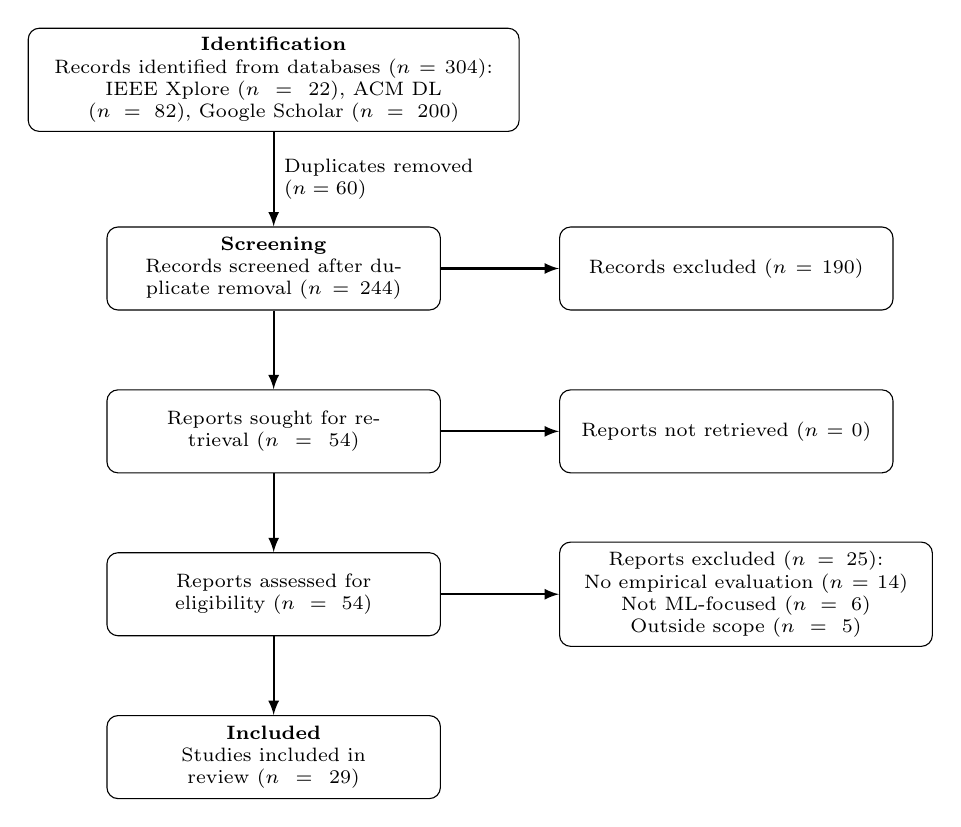
\begin{tikzpicture}[
    node distance=0.8cm and 1cm,
    box/.style={draw, rectangle, rounded corners, align=center, fill=white, minimum height=3em, text width=4cm, font=\scriptsize},
    arrow/.style={-latex, thick}
]

% Main column
\node[box, text width=6cm] (ident) {\textbf{Identification}\\Records identified from databases ($n=304$):\\IEEE Xplore ($n=22$), ACM DL ($n=82$), Google Scholar ($n=200$)};

\node[box, below=1.2cm of ident] (screen) {\textbf{Screening}\\Records screened after duplicate removal ($n=244$)};

\node[box, below=1.0cm of screen] (sought) {Reports sought for retrieval ($n=54$)};

\node[box, below=1.0cm of sought] (elig) {Reports assessed for eligibility ($n=54$)};

\node[box, below=1.0cm of elig] (inc) {\textbf{Included}\\Studies included in review ($n=29$)};

% Exclusions (Right side)
\node[box, right=1.5cm of screen] (exc_screen) {Records excluded ($n=190$)};

\node[box, right=1.5cm of sought] (not_ret) {Reports not retrieved ($n=0$)};

\node[box, right=1.5cm of elig, text width=4.5cm] (exc_full) {Reports excluded ($n=25$):\\No empirical evaluation ($n=14$)\\Not ML-focused ($n=6$)\\Outside scope ($n=5$)};

% Arrows
\draw[arrow] (ident) -- node[right, font=\scriptsize, align=left] {Duplicates removed\\($n=60$)} (screen);
\draw[arrow] (screen) -- (sought);
\draw[arrow] (sought) -- (elig);
\draw[arrow] (elig) -- (inc);

\draw[arrow] (screen) -- (exc_screen);
\draw[arrow] (sought) -- (not_ret);
\draw[arrow] (elig) -- (exc_full);

\end{tikzpicture}
\caption{PRISMA 2020 flow diagram of study selection process.}
\label{fig:prisma}
\end{figure*}
    

Common reasons for exclusion at full-text stage are detailed in Figure~\ref{fig:prisma}.

\subsection{Risk of Bias in Studies}
Using the adapted QUADAS-2 criteria (Table~\ref{tab:quadas2}), the included studies were classified as:
\begin{table}[t]
\centering
\small
\begin{tabular}{l r l}
\toprule
\textbf{Risk of Bias} & \textbf{n (\%)} & \textbf{Examples} \\
\midrule
Low & 12 (41\%) & Shokri et al.; Carlini et al. \\
Moderate & 14 (48\%) & Most FL+DP studies \\
High & 3 (10\%) & Synthetic-only studies \\
\bottomrule
\end{tabular}
\caption{Risk of bias distribution across included studies ($n=29$).}
\label{tab:risk_of_bias}
\end{table}

\subsection{Study Characteristics}
Table~\ref{tab:included_studies} summarizes representative included studies (selected examples) across threat and defense categories.

\begin{table*}[!t]
\centering
\scriptsize
\renewcommand{\arraystretch}{1.05}
\begin{tabular}{L{2.9cm} C{0.9cm} L{1.6cm} L{1.0cm} L{1.8cm} L{3.3cm} L{1.4cm}}
\toprule
\textbf{Authors (Year)} & \textbf{Threat} & \textbf{Defense} & \textbf{Model} & \textbf{Dataset} & \textbf{Privacy Metric} & \textbf{Utility Loss} \\
\midrule
Shokri et al. (2017)~\cite{shokri2017membership} & MI & None & NN & Purchase & Attack AUC 0.91 & Baseline \\
Nasr et al. (2019)~\cite{nasr2019comprehensive} & MI & DP-SGD & CNN & CIFAR-10 & Attack AUC 0.65 & --12\% acc \\
Carlini et al. (2021)~\cite{carlini2021extracting} & Extraction & None & GPT-2 & WebText & 1.3\% extraction & Baseline \\
Xiao et al. (2023)~\cite{xiao2023secure} & Infer & FL+SecAgg & -- & EDM & Info leak $\approx 0$ & --4\% AUC \\
\bottomrule
\end{tabular}
\caption{Characteristics of included studies (selected examples). MI=Membership Inference.}
\label{tab:included_studies}
\end{table*}

\begin{table}[!t]
\centering
\small
\begin{tabular}{l r r}
\toprule
\textbf{Category} & \textbf{n} & \textbf{\%} \\
\midrule
\textbf{Threat Type} & & \\
Membership Inference & 14 & 48\% \\
Model Inversion & 5 & 17\% \\
Data Extraction & 4 & 14\% \\
Multi-threat & 6 & 21\% \\
\midrule
\textbf{Defense Type} & & \\
Differential Privacy & 12 & 41\% \\
Federated Learning & 9 & 31\% \\
SMPC/Encryption & 4 & 14\% \\
Anonymization & 3 & 10\% \\
Other & 1 & 4\% \\
\midrule
\textbf{Domain} & & \\
General ML & 16 & 55\% \\
Healthcare & 7 & 24\% \\
Education & 3 & 10\% \\
Finance & 2 & 7\% \\
Other & 1 & 4\% \\
\bottomrule
\end{tabular}
\caption{Distribution of included studies by threat type, defense type, and application domain ($n=29$).}
\label{tab:distribution}
\end{table}

\subsection{Threat Landscape: Disclosure Attacks}

\subsubsection{Membership Inference Attacks}
\textbf{Threat model}: attackers query model predictions (black-box) or use gradients/weights (white-box) and leverage auxiliary data from a similar distribution to train shadow models. \textbf{Success metric}: ROC-AUC $>0.6$ or attack accuracy $>60\%$.

\textbf{Empirical findings} (14 studies): black-box attacks report AUC 0.65--0.91 (median 0.82), while white-box attacks report AUC 0.75--0.95 (median 0.88)~\cite{shokri2017membership,nasr2019comprehensive}. Vulnerability factors include overfitting, minority classes, and small datasets.

\subsubsection{Model Inversion Attacks}
\textbf{Threat model}: attackers have white-box access and optimize input reconstructions to maximize model confidence. \textbf{Success metric}: reconstruction quality (e.g., SSIM $>0.3$ for images; BLEU $>0.2$ for text), or sensitive attribute inference accuracy.

\textbf{Empirical findings} (5 studies): across the reviewed evaluations, inversion success varies by modality and access assumptions. Image-based settings (including medical imaging) report moderate reconstruction fidelity, while attribute inference can be substantially better when models expose confidence scores or gradients~\cite{fredrikson2015model}.

\subsubsection{Training Data Extraction}
Training data extraction targets memorization in generative models, including LLMs, to recover verbatim or near-verbatim training sequences~\cite{carlini2021extracting}. Reported extraction rates vary widely depending on sequence rarity, sampling strategies, and access constraints.

\subsubsection{Large Language Models: Training Data Extraction \& Prompt Injection}
Recent studies highlight three LLM-specific disclosure vectors:
\begin{itemize}
  \item \textbf{Training data extraction} (4 studies): crafted prompts trigger memorization~\cite{carlini2021extracting,huang2024training}; reported extraction rates range from 1.3\% to 40\% depending on sequence rarity and query strategy.
  \item \textbf{Prompt injection leading to disclosure} (3 studies): malicious prompts can bypass safeguards and extract system prompts or retrieved documents~\cite{zhu2023prompt,owasp_llm01}.
  \item \textbf{RAG/retrieval leakage} (excluded from core analysis): retrieval-augmented generation systems can leak private documents via prompt injection; we note this as an important real-world risk but outside the training-data scope of this review.
\end{itemize}

\subsection{Defense Mechanisms: Mitigation Strategies}

\subsubsection{Differential Privacy}
Differential privacy provides formal guarantees by limiting how much any single record can influence model outputs. In practice, DP-SGD adds noise to clipped gradients during training~\cite{abadi2016deep}. Stronger privacy (smaller $\varepsilon$) generally reduces utility, and careful accounting is needed under composition.

\subsubsection{Federated Learning, Secure Aggregation, and SMPC}
Federated learning reduces exposure by training across decentralized clients, but updates can still leak information via gradient-based attacks~\cite{geiping2020inverting}. Combining FL with secure aggregation, SMPC, and/or DP reduces leakage at additional computation and communication cost~\cite{xiao2023secure,wang2023federated}.

\subsubsection{Anonymization and Pseudonymization}
De-identification removes direct identifiers and masks quasi-identifiers to reduce re-identification risk. However, linkage attacks can still succeed, and utility can degrade, particularly for high-dimensional behavioral educational data.

\FloatBarrier
\section{Discussion}

\subsection{Answering RQ1: Threat Landscape}
Our synthesis of 29 studies reveals four primary data disclosure threats, ordered by prevalence:
\begin{enumerate}
  \item \textbf{Membership inference} (48\% of studies): most mature threat model and widest empirical evidence base.
  \item \textbf{Model inversion} (17\%): concentrated in specific modalities and domains (e.g., medical imaging).
  \item \textbf{Training data extraction} (14\%): LLM-focused and rapidly growing.
  \item \textbf{Multi-threat evaluations} (21\%): combined attack scenarios that better approximate real deployments.
\end{enumerate}

\subsection{Answering RQ2: Mitigation Approaches and Trade-offs}
Across included studies, defenses cluster into a small number of dominant approaches:
\begin{itemize}
  \item \textbf{Differential privacy} (41\%): commonly reported with $\varepsilon \in [1,10]$ and utility loss in the 5--15\% range, depending on dataset and model~\cite{abadi2016deep,li2024differentially}.
  \item \textbf{Federated learning} (31\%): reduces raw-data exposure but introduces communication overhead and non-IID training challenges; requires additional protections (DP, secure aggregation) to mitigate gradient leakage.
  \item \textbf{SMPC/encryption} (14\%): strong protection but often prohibitive computational cost.
  \item \textbf{Anonymization} (10\%): easy to deploy but weaker formal guarantees and vulnerable to linkage attacks.
\end{itemize}

\subsection{The Education Gap}
Only 3 of 29 studies focused explicitly on education~\cite{yu2024privacy,xiao2023secure,gursoy2022privacy}. This is a key gap given the sensitivity of student data and regulatory constraints. Existing educational studies predominantly evaluate federated learning and aggregation/anonymization approaches, with limited direct evaluation of membership inference and inversion risks on student predictive models.

\subsection{Methodological Gaps and Limitations}
Key limitations include the lack of standardized benchmarks, heterogeneous privacy metrics, and inconsistent reporting of statistical uncertainty and reproducibility artifacts. Single-reviewer screening also increases the risk of selection bias; this was mitigated through predefined PICOS criteria and documented exclusion decisions.

\subsection{Future Research Directions}
Future work should prioritize standardized privacy evaluation frameworks, more empirical studies in educational settings, and practical defenses for LLM disclosure risks (especially extraction and prompt-injection-driven disclosure).

\section{Conclusion}
\label{sec:Conclusion}
Data disclosure in AI/ML systems remains a significant and evolving threat landscape. This review synthesizes empirical evidence on disclosure attacks (membership inference, model inversion, and training data extraction) and defenses (differential privacy, federated learning, secure aggregation, and anonymization) across domains, with emphasis on educational applications. While formal privacy-preserving techniques are increasingly deployable, substantial trade-offs in utility and deployment complexity persist. The educational sector remains comparatively under-researched relative to healthcare and general benchmarks, underscoring the need for domain-specific empirical evaluations and more standardized reporting practices.

\nocite{*}
\bibliographystyle{IEEEtran}
\bibliography{references}
\end{document}